\section{Orderings that did not survive, and the pre-declared window average}
\label{sec:failed}

Table~\ref{tab:orderings2} lists the orderings we read off our measurements and then lost to
their own intervals, to a null control, to a partial correlation or to a matched grid.

% GENERATED FILE -- do not edit by hand.
% Rebuild:  python make_all.py (generator: make_orderings_v3.py)
% Appendix C, Table 11 (rewrite v3): make_orderings_v3.py, self-contained; reads no fold_average.json.
\begin{table}[htbp]
\centering
\caption{\textbf{Orderings that did not survive their own error bars.} Each row gives an ordering as we first read it and how it failed. The section column points to where it is discussed; --- marks those reported here only. Rows 1 and 5--8 are computed on the cleaned test pool and row 2 on the original test pool (Section~\ref{sec:testpool}); rows 3, 4 and 9 use no test data.}
\label{tab:orderings2}
\footnotesize
\setlength{\tabcolsep}{4pt}
\begin{tabular}{p{0.3\textwidth}lp{0.52\textwidth}}
\toprule
Ordering as first read & Section & How it failed \\
\midrule
1. The budget at which the self-training arm's curve peaks & \S\ref{sec:negative} & On the development fold the peak cannot be located: the steps within two positives of the best are \rwFzSteps{}, and \rwFzWithinSd{} of \rwFzPoints{} checkpoints lie within one sd of it. \\
\addlinespace
2. Decay sets in before the 8000-step cap & \S\ref{sec:negative} & Detectable only at the full cap of 8000; every shorter truncation (1500--6000) has an interval that crosses zero. \\
\addlinespace
3. Source--target agreement at initialisation predicts which feature directions the alignment objective shrinks & --- & Spearman $\rho = -0.76$ at the weight used, but $-0.90$ at weight zero, where the objective contributes no gradient; controlling for initial scale leaves $\rho = -0.002$. \\
\addlinespace
4. A Fisher-ratio separability measure rises with the alignment weight & --- & Monotone in the weight at whitening shrinkage 0.01 and 0.1; at 0.5 the weight-1 arm exceeds the weight-4 arm, so the ordering depends on the shrinkage. \\
\addlinespace
5. The ranking of the three unfrozen adaptation arms, under the choice of read-off step & App.~\ref{sec:resolution-fix} & At a single checkpoint DANN is first of three at step 2000 ($0.555$) and last at 4000 ($0.499$). Under the declared 8-checkpoint score average of logits the order is FreeMatch $\geq$ DANN $\geq$ CORAL at both, so the inversion came from reading a single checkpoint. \\
\addlinespace
6. DANN's across-fold spread exceeds the other arms' & --- & Holds at declared budgets ($0.1706$ against FreeMatch's $0.0697$). Budget-matched it shrinks against CORAL at 2000 ($0.1125$ against $0.0751$) and reverses against FreeMatch at 1500 ($0.0255$ against $0.0697$): it tracks training length. \\
\addlinespace
7. Folds 3 and 4 are intrinsically hard at the ranking level & --- & The self-training arm's AUROC on folds 3 and 4 ($0.969$, $0.971$) is above its fold 1 ($0.950$), so the difficulty is not a property of those folds alone. \\
\addlinespace
8. Unfreezing without an adaptation term is the least stable arm & --- & Holds on steps 250--8000 ($0.259$ against DANN's $0.199$; $0.131$ against $0.070$ after averaging) but not on the grid-matched 250--4000 after averaging ($0.025$ against $0.085$), so the order depends on the step range. \\
\addlinespace
9. The budget rule's crossing step is fixed by the trajectory & --- & The closest reading below the ceiling, at step 325, falls $0.025$ short; one sharper batch there would have set the budget at 650 steps instead of 1000, 35\% lower. \\
\bottomrule
\end{tabular}
\end{table}


\paragraph{BNM's carried-over predictions.} BNM's pre-registration carried two predictions
forward unrevised. We predicted that its late checkpoints would score lower than its earlier
ones, by too little to detect over \bnmDecayCap{} steps; on the development fold, the only
\bnmDecayCap{}-step run, and on the original test pool, the difference (earlier minus late) is
$\bnmDecayDelta{}$ $[\bnmDecayLo{}, \bnmDecayHi{}]$, undetectable but of the opposite sign. We
predicted that its predicted-positive fraction on the balanced target would rise from
\bnmPredPosStart{} toward \bnmPredPosTarget{} without collapsing; on folds 1--4 it had risen by
the first logged step, \bnmPredPosFirstStep{}, and then stayed between \bnmPredPosMin{} and
\bnmPredPosMax{}, with a mean of \bnmPredPosLate{} over the logged steps after
\bnmPredPosLateFrom{}, and it did not collapse. Each prediction held only in part.

\paragraph{The pre-declared window average.}
\label{sec:resolution-fix}
\label{sec:resolution-diagnosis}
Before computing any windowed number, we declared and hashed a secondary analysis: average the
per-example scores of the $k$ consecutive checkpoints ending at each arm's read-off step, for
$k \in \{1, 2, 4, 8\}$, under two score combinations. It replaces no pre-registered read-off.
Table~\ref{tab:window2} reports it; $k=1$ reproduces each arm's headline. Checkpoints are \ckptFm{} steps apart for FreeMatch and \ckptOther{} for the other arms, so a full $k=8$ window spans \winEightSpanFm{} training steps for FreeMatch and \winEightSpanOther{} for the others. At $k=8$ the order of
the three unfrozen adaptation arms no longer depends on which of DANN's two read-off steps is
used (the fifth row of Table~\ref{tab:orderings2}), but the two score combinations place DANN
and CORAL in opposite orders.

% GENERATED FILE -- do not edit by hand.
% Rebuild:  python make_all.py (generator: make_appendix_relabel_v2.py)
% Relabelled copy of tables/T6_window.tex; tabular number tokens asserted identical, caption/notes token changes declared.
\begin{table}[htbp]
\centering
\caption{\textbf{Checkpoint-window score averaging.} Fold-mean TPR@$10^{-3}$ when the per-example scores of the $k$ consecutive checkpoints ending at each arm's read-off step are averaged. We declared $k \in \{1, 2, 4, 8\}$, both score combinations and the window placement, and hashed them (\texttt{a572b81e\ldots}), before computing any windowed number. This is a secondary analysis and replaces no pre-registered read-off. $k=1$ reproduces each arm's headline. $k_{\mathrm{ach}}$ is the achieved window where fewer than $k$ checkpoints exist before the read-off; the window truncates rather than padding. Checkpoints are \ckptFm{} steps apart for FreeMatch and \ckptOther{} for the other arms, so a full $k=8$ window spans \winEightSpanFm{} training steps for FreeMatch and \winEightSpanOther{} for the others. At $k=8$ the two combinations order CORAL and DANN differently. Rows are folds 1--4 except Baseline~A$^{\dagger}$, a single model averaged over folds 0--4 and computed on the original test pool.}
\label{tab:window2}
\footnotesize
\setlength{\tabcolsep}{4pt}
\begin{tabular}{lrrrrrrrrrr}
\toprule
 & & & \multicolumn{4}{c}{mean logit (primary)} & \multicolumn{4}{c}{mean rank (secondary)} \\
\cmidrule(lr){4-7}\cmidrule(lr){8-11}
Arm & Read at & $k_{\mathrm{ach}}$ & $k{=}1$ & $k{=}2$ & $k{=}4$ & $k{=}8$ & $k{=}1$ & $k{=}2$ & $k{=}4$ & $k{=}8$ \\
\midrule
CORAL & 2000 & 8 & $0.5216$ & $0.5626$ & $0.5472$ & $0.5472$ & $0.5216$ & $0.5498$ & $0.5319$ & $0.5191$ \\
FreeMatch & 1500 & 8 & $0.5167$ & $0.5269$ & $0.5780$ & $0.5933$ & $0.5167$ & $0.5247$ & $0.5681$ & $0.5779$ \\
DANN & 4000 & 8 & $0.4985$ & $0.5446$ & $0.5573$ & $0.5573$ & $0.4985$ & $0.5166$ & $0.4986$ & $0.4755$ \\
DANN\,\footnotesize(sens.) & 2000 & 8 & $0.5547$ & $0.5753$ & $0.5600$ & $0.5498$ & $0.5547$ & $0.5424$ & $0.4935$ & $0.4680$ \\
$\lambda=0$ & 4000 & 8 & $0.1842$ & $0.2097$ & $0.2021$ & $0.2302$ & $0.1842$ & $0.2047$ & $0.2022$ & $0.2148$ \\
$\lambda=0$\,\footnotesize(sens.) & 2000 & 8 & $0.2149$ & $0.2200$ & $0.2302$ & $0.2814$ & $0.2149$ & $0.2175$ & $0.2302$ & $0.2737$ \\
$\lambda=0$\,\footnotesize(sens.) & 1500 & 6 & $0.1944$ & $0.2147$ & $0.2557$ & $0.2661$ & $0.1944$ & $0.2147$ & $0.2506$ & $0.2737$ \\
BNM\,\footnotesize(own budget) & 1000 & 4 & $0.4196$ & $0.4298$ & $0.4297$ & $0.4297$ & $0.4196$ & $0.4067$ & $0.4067$ & $0.4067$ \\
BNM\,\footnotesize(sens.) & 1500 & 6 & $0.3833$ & $0.4166$ & $0.4193$ & $0.4245$ & $0.3833$ & $0.3987$ & $0.4167$ & $0.4066$ \\
BNM\,\footnotesize(sens.) & 2000 & 8 & $0.4041$ & $0.4424$ & $0.4295$ & $0.4398$ & $0.4041$ & $0.4092$ & $0.4040$ & $0.3989$ \\
BNM & 4000 & 8 & $0.4040$ & $0.4322$ & $0.4475$ & $0.4705$ & $0.4040$ & $0.4117$ & $0.4143$ & $0.4193$ \\
Baseline A$^{\dagger}$ & 8000 & 8 & $0.1759$ & $0.1718$ & $0.1657$ & $0.1637$ & $0.1759$ & $0.1739$ & $0.1698$ & $0.1657$ \\
\bottomrule
\end{tabular}

\vspace{2pt}
\footnotesize $^{\dagger}$Baseline A's per-step scores are recomputed on CPU from the frozen 640-d feature cache and the retained per-step head weights, which is exact because the encoder is frozen.
\end{table}


\paragraph{The declaration's other outputs.} Table~\ref{tab:window-secondary} gives the two
secondary metrics the declaration named. The declaration also asked whether averaging reduces
the checkpoint scatter by the $\sqrt{k}$ expected of independent checkpoints: at $k=8$ it
reaches \winSqrtkLam{} of that for the control and \winSqrtkMin{}--\winSqrtkMax{} for the other
arms (CORAL's checkpoint grid allows the test only up to $k=4$, where it reaches
\winSqrtkCoral{}), consistent with checkpoint noise that is correlated across checkpoints for
the control and CORAL. It also asked whether each ordering that a read-off choice could have
caused survives the averaging. Besides the read-off inversion above, three such orderings have
a verdict. DANN's across-fold spread is still the widest at $k=8$ on the cleaned pool
(\winSixDann{} against CORAL's \winSixCoral{}), but not on the original pool, where BNM's is
(\winSixBnmOrig{} against DANN's \winSixDannOrig{}). At $k=8$ the within-run checkpoint scatter
is \winEightSdLo{} to \winEightSdHi{}, still \winEightMultLo{} to \winEightMultHi{} times the
\winEightDiff{} difference between DANN and CORAL that we first read on the original pool. And
on folds 1--4 the control's range across checkpoints is narrower than DANN's at both $k=1$ and
$k=8$, so it is not the least stable arm there.

% GENERATED FILE -- do not edit by hand.
% Rebuild:  python make_all.py (generator: make_prereg_fixes.py)
% Appendix C: the window declaration's secondaries, from paper/data/window_average_D1.json.
\begin{table}[htbp]
\centering
\caption{\textbf{The window average's secondary metrics.} Fold-mean AUROC and completeness at 24\% purity, folds 1--4, cleaned pool, for a single checkpoint ($k=1$, each arm's headline) and for the declared eight-checkpoint average under each score combination. The declaration named both metrics as secondaries (Table~\ref{tab:window2} gives TPR). \emph{n/a}: 24\% purity is unreachable on at least one fold.}
\label{tab:window-secondary}
\footnotesize
\setlength{\tabcolsep}{4pt}
\begin{tabular}{lrrrrrrr}
\toprule
 & & \multicolumn{3}{c}{AUROC} & \multicolumn{3}{c}{completeness at 24\% purity} \\
\cmidrule(lr){3-5}\cmidrule(lr){6-8}
Arm & Read at & $k{=}1$ & $k{=}8$, logit & $k{=}8$, rank & $k{=}1$ & $k{=}8$, logit & $k{=}8$, rank \\
\midrule
CORAL & 2000 & $0.9097$ & $0.9423$ & $0.9369$ & $0.4961$ & $0.5421$ & $0.4884$ \\
FreeMatch & 1500 & $0.9666$ & $0.9756$ & $0.9735$ & $0.4835$ & $0.5677$ & $0.5626$ \\
DANN & 4000 & $0.9076$ & $0.9540$ & $0.9451$ & $0.4550$ & $0.5394$ & $0.4679$ \\
DANN\,\footnotesize(sens.) & 2000 & $0.9326$ & $0.9539$ & $0.9513$ & $0.5291$ & $0.5166$ & $0.4194$ \\
$\lambda=0$ & 4000 & $0.8815$ & $0.8935$ & $0.8922$ & \emph{n/a} & $0.0587$ & $0.0715$ \\
BNM & 4000 & $0.9096$ & $0.9234$ & $0.9155$ & $0.3555$ & $0.4397$ & $0.3682$ \\
\bottomrule
\end{tabular}
\end{table}


\paragraph{Paired contrasts after the window average.} Table~\ref{tab:k8pairs6} gives the
\rwFiveKPairsWord{} pairs among CORAL, DANN and FreeMatch at their declared read-offs, at $k=1$
and at $k=8$ under both score combinations. FreeMatch has the highest $k=8$ fold-mean under
both; its lead excludes zero under mean rank and not under mean logit
(Section~\ref{sec:resolution}).

% GENERATED FILE -- do not edit by hand.
% Rebuild:  python make_all.py (generator: make_dilute10_tables.py)
% Paper v6: tables/C_k8_pairs.tex unchanged except 1 reference(s) to Table 2 (tab:contrasts2 -> tab:contrasts6) and its label (tab:k8pairs -> tab:k8pairs6).
\begin{table}[tbp]
\centering
\caption{\textbf{Paired contrasts among the three unfrozen adaptation arms} at each arm's declared read-off ($k=1$) and after the pre-declared $k=8$ window average, folds 1--4, cleaned pool, paired $t$ ($\mathrm{df}=3$). At $k=1$ the two score combinations coincide. Computed after the results were known, from the declared window rule; ten further intervals at $k=8$, and two at $k=1$ that Table~\ref{tab:contrasts6} does not report, all without multiplicity correction. Each pair's first line gives $\Delta$ and the signs, the folds agreeing in direction with the mean; the second line gives the 95\% interval. $^{*}$Interval excludes zero.}
\label{tab:k8pairs6}
\scriptsize
\setlength{\tabcolsep}{2pt}
\begin{tabular}{llrcrcrc}
\toprule
 & & \multicolumn{2}{c}{$k=1$} & \multicolumn{2}{c}{$k=8$, mean logit (primary)} & \multicolumn{2}{c}{$k=8$, mean rank (secondary)} \\
\cmidrule(lr){3-4}\cmidrule(lr){5-6}\cmidrule(lr){7-8}
Pair & Steps & $\Delta$ (95\% CI) & Signs & $\Delta$ (95\% CI) & Signs & $\Delta$ (95\% CI) & Signs \\
\midrule
DANN $-$ CORAL & 4000 / 2000 & $-0.0231$ & 2/4 & $+0.0100$ & 3/4 & $-0.0436$ & 3/4 \\
 &  & $[-0.2227, +0.1765]$ &  & $[-0.0833, +0.1034]$ &  & $[-0.1251, +0.0379]$ &  \\
\addlinespace
DANN $-$ CORAL & 2000 / 2000 & $+0.0331$ & 2/4 & $+0.0026$ & 2/4 & $-0.0511$ & 4/4 \\
 &  & $[-0.0711, +0.1372]$ &  & $[-0.0587, +0.0639]$ &  & $[-0.1073, +0.0051]$ &  \\
\addlinespace
DANN $-$ FreeMatch & 4000 / 1500 & $-0.0182$ & 2/4 & $-0.0360$ & 3/4 & $-0.1024$$^{*}$ & 4/4 \\
 &  & $[-0.2092, +0.1729]$ &  & $[-0.1312, +0.0592]$ &  & $[-0.1327, -0.0720]$ &  \\
\addlinespace
DANN $-$ FreeMatch & 2000 / 1500 & $+0.0380$ & 3/4 & $-0.0435$ & 4/4 & $-0.1099$$^{*}$ & 4/4 \\
 &  & $[-0.1148, +0.1908]$ &  & $[-0.0987, +0.0118]$ &  & $[-0.1520, -0.0677]$ &  \\
\addlinespace
CORAL $-$ FreeMatch & 2000 / 1500 & $+0.0049$ & 2/4 & $-0.0460$ & 3/4 & $-0.0588$$^{*}$ & 4/4 \\
 &  & $[-0.0933, +0.1032]$ &  & $[-0.0999, +0.0078]$ &  & $[-0.1106, -0.0069]$ &  \\
\bottomrule
\end{tabular}
\end{table}


\paragraph{Checkpoint noise under an independence assumption.} Figure~\ref{fig:resolution}
sets each gap between two adaptation arms against the contribution checkpoint-to-checkpoint
scatter would make to it if the two arms' checkpoint noise were independent. Under that
assumption the gaps among CORAL, DANN and FreeMatch, between $\rvGapThreeMin{}$ and
$\rvGapThreeMax{}$, are smaller than the noise, and the gaps between BNM and each of them,
between $\rvGapBnmMin{}$ and $\rvGapBnmMax{}$, are larger; the largest noise figure is about
$\rvScale{}$. BNM $-$ CORAL is the one comparison between objectives whose single-checkpoint
interval excludes zero (Table~\ref{tab:contrasts6}). We made this analysis after the results
were known. For at least one pair the independent noise figure exceeds the standard error the
paired interval implies, so it overstates the noise in a paired comparison
(Section~\ref{sec:resolution}).

\begin{figure}[t]
\centering
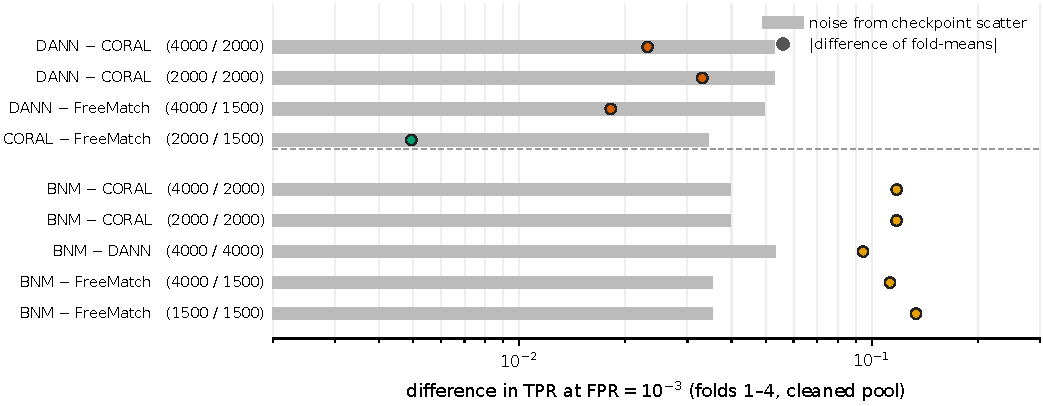
\includegraphics[width=\textwidth]{F5_resolution_v2.pdf}
\caption{\textbf{Differences between methods against checkpoint noise.} For each pair of
adaptation arms read at declared read-offs, the bar is the contribution of
checkpoint-to-checkpoint scatter to a difference of four-fold means, and the point is the
difference of the fold-means; log axis. As computed here, the gaps among CORAL, DANN and
FreeMatch (top) lie inside the noise and the gaps between BNM and each of them (bottom) lie
outside it. The bars assume
that the two arms' checkpoint noise is independent, which overstates it
(Section~\ref{sec:resolution}).}
\label{fig:resolution}
\end{figure}
